\chapter{Replication: Copying Billions of Letters}

\begin{kaichang}
You accidentally nick a finger while chopping vegetables. Rinse it, apply an adhesive bandage, and look again a few days later: the scab has fallen away, new skin has grown underneath, and even the fingerprint ridges look almost as before.

Now guess two things. First, how many new cells did your body make to repair that little cut? Second, every new cell contains a complete hereditary instruction manual---three billion ``letters,'' or bases, in the human version. Where did those letters come from? Did the new cell invent them, or copy them from an old cell? If copied, who did the copying, and how were mistakes prevented?

Write down your guesses. We will return to the wound at the end and discover the immense copying project that just unfolded beneath it.
\end{kaichang}

\textbf{Translator safety note:} This is an illustrative account, not a reason to make a cut or assume every wound heals unaided. Seek medical advice for a deep, infected, worsening, or persistently bleeding wound; see \href{https://www.nhs.uk/conditions/cuts-and-grazes/}{NHS wound-care guidance}.

\section{Double First, Then Divide}

A wound heals as its edge cells divide: one becomes two, two become four, filling the gap. Chapter 64 introduced cell division: chromosomes are copied, then shared equally between daughter cells. Now zoom into one molecular step: how does chromosome DNA ``double first''?

Start with observable, measurable facts. Your nails grow roughly a millimeter weekly and your hair over a centimeter monthly; all that new growth consists of new cells. In a culture dish at $37\,^{\circ}\mathrm{C}$, one E. coli becomes two every twenty minutes or so. A fertilized egg divides for dozens of rounds to produce tens of trillions of cells. All share one strict rule: \textbf{before division, the cell's total DNA must exactly double}. This can be measured directly: stain DNA with a fluorescent dye and measure its brightness under a microscope. A cell preparing to divide is exactly twice as bright as an ordinary one, no more or less.

Why exactly double? What if there is too much or too little? Each daughter cell needs a whole manual, without extra or missing pages. Omit a segment and a component's blueprint is missing; duplicate a segment unnecessarily and hereditary information goes awry. The cell therefore separates ``copy the book'' and ``divide the household'' into successive stages: first copy all three billion letters, then split in two.

But how do you copy three billion letters, who does it, and what happens to mistakes? Return to Chapter 66's double-helix blueprint.

\section{Each Strand Is the Other's Blueprint}

Recall the structure: two long strands wind together, joined by base pairing. Adenine (A) always faces thymine (T); guanine (G) always faces cytosine (C). Chapter 66 explained the strict chemistry: shapes and hydrogen-bond donor and acceptor positions allow only these partners to fit precisely into the helix.

Now consider an implication that seems ordinary but is astonishing: \textbf{knowing one strand's sequence completely determines the other}. Write A on one strand and the opposite must be T; write G and it must be C. The strands are like a photographic negative and its print: either lets you develop the other anew.

Watson and Crick ended their 1953 paper with a sentence quoted ever since: ``We have noticed that the pairing we propose directly suggests a possible copying mechanism for hereditary material.'' They meant this: unzip the strands, use each as a template, and install new bases one by one according to the rules---T opposite A, C opposite G. One original double helix becomes two, each containing one old and one new strand.

Wait: must each contain one old and one new strand? Not necessarily. At least three copying schemes are logically plausible:

\begin{itemize}[itemsep=2pt]
\item \textbf{Semiconservative replication}: separate the old strands and give each a new partner. Both resulting DNA molecules are ``half old, half new.''
\item \textbf{Conservative replication}: keep the original helix intact and make a wholly new helix alongside it. One result is entirely new, the other entirely old.
\item \textbf{Dispersive replication}: fragment the old strands and mix their pieces with newly synthesized material. Every strand in both molecules is a ``patchwork quilt'' of old and new.
\end{itemize}

All three double DNA and respect complementary pairing. Biologists argued for years in the 1950s without persuading one another: this was precisely the sort of question thought alone cannot settle. Experiment must vote. We will examine that vote in the evidence section; first understand the copying itself.

\begin{shiyan}
\textbf{Fish Out DNA Yourself.} DNA is not an abstract textbook symbol but a real long molecule, long enough for your naked eye to see---provided you collect enough molecules at once.

Materials: two or three strawberries (or half a banana), a small spoonful of salt, a few drops of dishwashing liquid, water, gauze or a coffee filter, two clear cups, and a small cup of chilled high-strength alcohol, such as vodka or baijiu, supplied by a parent.

Steps: Remove the strawberry tops, put the fruit in a food-storage bag, add two spoonfuls of water, a pinch of salt, and a few drops of detergent. Gently mash through the bag and leave for five minutes. Filter the pulp into a cup, retaining a little under half a cup of filtrate. Slowly pour cold alcohol down the cup wall so it floats above the liquid without stirring. Watch the interface.

Observations: White strands appear within minutes and can be wound around a toothpick. They are thousands upon thousands of tangled DNA molecules, mixed with some protein. Salt and detergent break apart membranes and proteins; DNA is insoluble in cold alcohol and aggregates into a precipitate. Consider how, within a strawberry's cells, these ``strands'' were folded into spaces smaller than a pinhead.

Safety: Keep flammable alcohol away from ignition sources throughout. Do not eat treated experimental materials; wash your hands afterward. The experiment can be done at home, but a parent must dispense the alcohol.
\end{shiyan}

\textbf{Translator safety note:} Follow Chapter 66's alcohol precautions: do not put flammable chemicals in an ordinary refrigerator or freezer. A qualified teacher should choose a safe preparation and chilling procedure; an adult handles alcohol, with eye protection and no tasting or ignition sources. See \href{https://ehs.stanford.edu/wp-content/uploads/Lab-Compliance-Cheat-Sheet.pdf}{Stanford storage guidance} and \href{https://www.acs.org/education/celebrating-chemistry-editions/2024-ccew/science-safety-tips.html}{ACS activity precautions}.

\section{A Copying Crew with Clear Roles}

Pairing determines ``what to copy,'' but enzymes perform the work. There is no scribe's desk inside a cell, only protein machines running along DNA like an assembly-line construction crew. Meet the main workers.

\textbf{Helicase} clears the way. It grips the helix and consumes ATP (Chapter 52's energy currency) to pull apart interstrand hydrogen bonds, opening a Y-shaped \textbf{replication fork}, the copying worksite. Remember, the strands wind around each other: unwinding here twists the region farther ahead ever tighter, like knots in a wrung towel. Another enzyme therefore relieves the twisting stress farther ahead.

\textbf{Primase} lays the first brick. The copying enzyme, DNA polymerase, has an important quirk: it \textbf{cannot start from scratch}, only add bases to the end of an existing strand. Before each segment begins, primase synthesizes a short RNA ``starting platform,'' onto which subsequent bases are added. The platform is later removed and the gap filled with DNA.

\textbf{DNA polymerase} does the main copying. Sliding along the template and reading bases individually, it selects matching building blocks from the cytoplasmic supply of four deoxynucleotides, each carrying three phosphates, and clicks them onto the new strand's end. Energy for attachment comes from the chemical energy released when the substrate sheds two phosphates. Notice: bond formation and hydrolysis release energy overall; energy is not ``hidden inside a high-energy bond,'' as Chapter 52 clarified.

\textbf{Ligase} is the finishing mason, sealing gaps in the new strand. Why is it necessary? That brings us to replication's most awkward design.

Polymerase also has an unchangeable directional preference: it works only one way. But DNA's strands are antiparallel (Chapter 66), and the fork continually opens forward. On one template, the new strand can follow the fork continuously: the \textbf{leading strand}. On the other, polymerase must work away from the fork's advance, ``building backward'' in short segments. After finishing one, it returns near the fork, lays another primer, and copies the next. This discontinuous product is the \textbf{lagging strand}; its short segments are Okazaki fragments, named for Japanese scientist Reiji Okazaki and his wife, their discoverers. Every fragment begins with a primer to remove and leaves gaps to seal, making the lagging strand particularly laborious. This is where ligase is especially busy.

\begin{qiaoliang}
How fast is this crew? A bacterial fork can add about 1000 bases per second. E. coli has roughly 4.6 million base pairs; two forks set out in opposite directions from one origin. Copying the chromosome takes $4.6\times10^{6}\div(2\times1000)\approx2300$ seconds, around forty minutes, broadly fitting its twenty-minute generation time. Its trick is to start the next round on unfinished copies before the previous round ends.

Human forks are much slower, about 50 bases per second. A single bidirectional origin would take almost two years to copy three billion base pairs. Yet a cell actually finishes in about eight hours. How? \textbf{Many worksites}: tens of thousands of origins are scattered along human chromosomes and activated in batches, with thousands or tens of thousands of forks working simultaneously. Slowness is manageable if there are enough worksites.
\end{qiaoliang}

\section{Mistakes: A Pencil with an Eraser}

The speed is impressive; the accuracy more so. Polymerase initially selects bases mainly by pairing geometry, but occasionally misjudges, inserting about one wrong letter in ten thousand to a hundred thousand. If accuracy stopped there, each genome copy would gain hundreds of thousands of spelling mistakes, with unimaginable consequences.

So polymerase carries an eraser: a ``proofreading'' site. A newly added mismatched base distorts the new end, making polymerase stall, back up, remove the base, and try again. This cuts errors to roughly one in ten million. After copying, a second defense patrols the DNA: \textbf{mismatch repair}, searching for escaped mismatches, identifying the new strand (cells can mark old and new), and removing and recopying the incorrect segment. Together, the checkpoints lower the final error rate to one letter in a billion to ten billion.

Imagine copying books by hand with permission for only one error per billion letters. You would need to copy over two thousand complete sets of Dream of the Red Chamber before earning one mistake. Cells achieve this through molecular ``write--check--repair,'' not luck.

But one in a billion is \textbf{not zero}. Across three billion base pairs, each cell division leaves a few new spelling differences on average. Every body cell's genome differs slightly from the fertilized egg's original. Remember this: it opens the way to several later chapters, and we will return to it before this one ends.

\section{Writing Replication in Symbols}

After all those machines, put copying itself into symbols. There are only two rules: pairing (A with T, G with C) and direction (the new strand always extends from $5'$ toward $3'$, while the template is read oppositely). For example, take this template:

\[3'-\mathrm{TACGGATC}-5'\]

Reading left to right, the copyist makes:

\[5'-\mathrm{ATGCCTAG}-3'\]

One letter opposite another, strands running in opposite directions: the practical consequence of Chapter 66's antiparallel structure, and the fundamental reason the lagging strand must ``build backward.'' Write any template yourself and produce its complement with these two rules. Congratulations: you have performed DNA polymerase's task with paper and pen, only a hundred million times slower.

Do not underestimate this alphabet. The entire hereditary manual has just four letters, meager beside English's twenty-six, yet their order stores all information needed to build a whole person. As Chapter 66 explained, information lies in the order, not the letters themselves. Replication protects that order: machines may be slow or take detours, but not one letter may move out of sequence.

\section{Three Copying Models: Experiment Votes}

\begin{zhengju}
Return to the mystery: semiconservative, conservative, or dispersive replication? In 1958, Meselson and Stahl at the California Institute of Technology devised what later became ``the most beautiful experiment in biology,'' settling the issue.

Their trick was to ``weigh'' DNA. Nitrogen is an important base component. Ordinary nitrogen is $\chem{^{14}N}$, but a stable heavier isotope, $\chem{^{15}N}$, also exists (Chapter 7 explained equal proton counts and different neutron counts). They grew E. coli for more than ten generations in medium containing only $\chem{^{15}N}$, making every DNA strand ``heavy.'' They then abruptly moved the bacteria to ordinary $\chem{^{14}N}$ medium, so new strands would be ``light.'' Sampling each generation, they extracted DNA and ultracentrifuged it in cesium chloride for more than ten hours. Centrifugal force forms a density gradient, lighter above and denser below. DNA floats at its matching density: heavy molecules lower, light ones higher, with bands visible under ultraviolet.

The models predict distinct outcomes. Conservative replication gives two bands in generation one: fully heavy old helices and fully light new ones. Dispersive replication gives one band every generation, progressively higher. Semiconservative replication gives one middle band first, each helix containing a heavy and a light strand; generation two splits it into equal middle and light bands.

The result: one middle band in generation one eliminated conservative replication. Equal middle and light bands in generation two eliminated dispersive replication. Meselson and Stahl later heated second-generation hybrid DNA into single strands and centrifuged again, obtaining a heavy and a light strand and sealing the case for ``one old, one new.'' The experiment relied not on a genius's flash, but on calculating the hypotheses' \textbf{observable consequences} in advance and letting centrifuge tubes vote.
\end{zhengju}

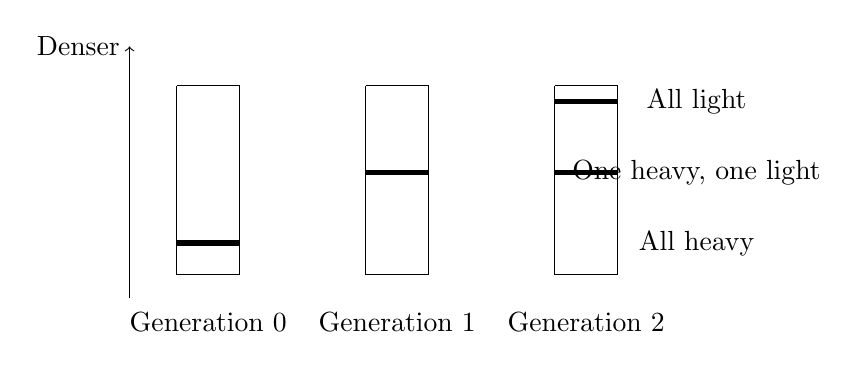
\begin{tikzpicture}
\draw[->] (-0.6,0) -- (-0.6,3.2) node[left]{Denser};
\foreach \x/\lab in {0/Generation 0, 2.4/Generation 1, 4.8/Generation 2}{
  \draw (\x,0.3) -- (\x,2.7);
  \draw (\x+0.8,0.3) -- (\x+0.8,2.7);
  \draw (\x,0.3) -- (\x+0.8,0.3);
  \draw (\x,2.7) -- (\x+0.8,2.7);
  \node at (\x+0.4,-0.3){\lab};
}
\draw[line width=2pt] (0,0.7) -- (0.8,0.7);
\draw[line width=2pt] (2.4,1.6) -- (3.2,1.6);
\draw[line width=2pt] (4.8,1.6) -- (5.6,1.6);
\draw[line width=2pt] (4.8,2.5) -- (5.6,2.5);
\node at (6.6,0.7){All heavy};
\node at (6.6,1.6){One heavy, one light};
\node at (6.6,2.5){All light};
\end{tikzpicture}

This is a schematic of centrifugation results, not an actual photograph; horizontal lines show DNA band positions. Notice the simultaneous middle and light bands in generation two: that alone excludes dispersive replication.

\section{Trouble at the End: Telomeres}

The copying machinery is nearly perfect, but has an inherent blind spot at chromosome ends.

Recall lagging-strand construction: each segment begins with an RNA primer, later removed and replaced by DNA. At the chromosome's very end, removing the last primer leaves \textbf{no space before it} for polymerase to begin filling in. Polymerase can only extend backward, not fill forward. Each replication therefore shortens this lagging-strand end a little. This ``end-replication problem'' follows inevitably from directional copying, not a machine failure.

The cell places a ``disposable safety helmet'' on each end: a \textbf{telomere}, thousands of noncoding repeats (human telomeres repeat TTAGGG thousands of times). Division wears away the helmet, not the blueprint text. Eventually, though, the helmet thins. After forty or fifty divisions in culture, human cells reach a critical telomere length and permanently stop dividing: the Hayflick limit. Chapter 60 described continual correction in homeostasis; telomeres show another side of that system, imposing a division allowance that prevents unlimited proliferation.

How, then, do germ cells and stem cells continue across generations? A specialized enzyme, \textbf{telomerase}, carries a short RNA template and replenishes the cap, whereas most ordinary body cells switch it off. Alarmingly, about ninety percent of cancer cells reactivate it, turning disposable helmets into permanent ones, one ticket to unlimited division. Telomerase thus supports life's continuity and is an important cancer-research target. The same key opens different doors depending on who holds it.

State the model's boundaries. Our main subject is nuclear-chromosome replication, simplified in mainstream textbook fashion. Real cells have multiple DNA polymerases, some initiating, some specializing in leading or lagging strands, rather than one generic copyist. Error rates vary with species, tissue, and age; one in a billion to ten billion is only an order of magnitude. Bacterial circular chromosomes lack ends and avoid telomere problems. Many viruses instead use RNA, with different copying rules and error rates (Chapter 65 introduced them; Chapter 79 returns to them). The main picture remains useful, but is no universal construction plan.

\begin{wuqu}
``Replication errors all come from external radiation and toxins; a clean environment makes copying perfectly accurate.'' Wrong. Even without any radiation or toxins, copying machinery makes initial errors around one in ten thousand, with roughly one in a billion escaping proofreading and repair. Copying three billion base pairs inevitably leaves a few new differences on average. Almost every cell dividing in your body today differs somewhat from the fertilized egg's original. Moreover, most errors matter less than you may imagine: most fall in noncoding sequence or do not affect protein function. The rare ones demanding concern hit crucial genes and evade repair. Whether mutation is error, raw material, or innovation is Chapter 72's topic.
\end{wuqu}

\section{Your Body's Total Copying Work}

Calculate a grand total to appreciate the scale. Roughly three hundred billion cells reach the end of life and are replaced daily, mainly blood and intestinal-lining cells. Every new cell requires a complete genome copy before taking its post. The human diploid genome contains about $6\times10^{9}$ base pairs, giving a daily total of:

\[3\times10^{11}\ \text{cells}\times 6\times10^{9}\ \text{base pairs}\approx 2\times10^{21}\ \text{letters}\]

What does $2\times10^{21}$ letters mean? Printed as characters in books, they could fill millions of libraries. This happens silently inside you, with errors kept extremely low. Life's daily maintenance bill exceeds intuition.

Medicine has borrowed the machinery in reverse. PCR (polymerase chain reaction), used in nucleic acid testing and forensic identification, transfers unwinding, pairing, and extension into a tube. Heating to about $95\,^{\circ}\mathrm{C}$ replaces helicase and separates DNA; cooling lets synthetic primers bind; a heat-resistant polymerase borrowed from hot-spring bacteria extends new strands. Each cycle doubles the target segment.

\begin{tiaozhan}
PCR doubling is exponential: starting from one copy, cycle $n$ gives $2^{n}$. Ten cycles yield about a thousand, twenty a million, thirty a billion ($2^{30}\approx1.07\times10^{9}$). Thus even a short nucleic-acid segment from a few viruses in a throat swab can become detectable after thirty-odd cycles. Exponential growth powerfully amplifies tiny signals. It also explains PCR laboratories' fear of contamination: one unwelcome molecule can likewise be amplified a billionfold. Use logarithms: how many cycles are needed to amplify one copy to at least $10^{12}$? (Hint: $\lg 2\approx0.30$.) You may skip this box without losing the thread.
\end{tiaozhan}

\section{Back to the Little Cut}

Now remove the bandage. As the cut healed, epithelial cells and fibroblasts at its edges worked overtime, dividing to fill it. Every new cell underwent a full copying operation: tens of thousands of origins started together; helicase opened DNA; primers laid the path; polymerase advanced at about 50 letters per second; proofreading erased errors; mismatch repair patrolled again; and ligase sealed every gap. A few hours, six billion letters, single-digit errors. Nearly restored fingerprint ridges reflect not luck but this ``write--check--repair'' line passing information almost unchanged.

Do not forget those single-digit errors or telomeres wearing with each division. Copying is highly reliable, not perpetual motion or absolute perfection. How cells handle miscopied text and bodies track divisions remains part of life's suspense.

A more fundamental question has been sidestepped throughout: what does each page of this three-billion-letter manual actually say? How does a cell turn one page's ``blueprint'' into a working protein? Copying preserves information; \textbf{using} it requires another process. First, a page of the master locked in the nucleus is transcribed into a portable work order. Next chapter, we follow that order.

\section*{Try It Yourself}

\begin{sikaoti}
\item Write any 12-letter DNA sequence using only A, T, G, and C. Label its $5'$ and $3'$ ends, then write the new strand copied from it with its direction. Exchange papers with your deskmate: do both pairing and direction obey the rules?
\item Draw a particle diagram of a replication fork: a Y-shaped opening, template strands, helicase, leading and lagging strands, and Okazaki fragments. Arrow each new strand's extension direction. Note that this is a thinking aid, not the molecules' actual appearance.
\item If replication were dispersive, what bands would appear in generations one, two, and three of Meselson--Stahl's experiment? Draw three ``tubes,'' compare them with actual semiconservative results, and identify which generation decisively distinguishes the models.
\item A human fork copies about 50 bases per second and S phase lasts about eight hours. Estimate one fork's total base pairs over S phase, then estimate how many origins must be used to copy a three-billion-base-pair genome, assuming each origin is used once. Show your calculations.
\item Somatic telomeres shorten each division, while cancer cells reactivate telomerase. Someone concludes that ``telomerase supplements bring immortality.'' Identify at least two leaps using this chapter's content and principles of dose and evidence, and explain possible risks.
\item Why must mismatch repair distinguish old from new strands? What happens if it wrongly ``corrects'' the old strand? Explain with an information-flow diagram: template→new strand→repair.
\end{sikaoti}
